\documentclass[times, utf8, zavrsni]{fer}
\usepackage{booktabs}
\usepackage{tikz}

\begin{document}

% TODO: Navedite broj rada.
\thesisnumber{253}

% TODO: Navedite naslov rada.
\title{Prebrojavanje razapinjućih stabala grafa}

% TODO: Navedite vaše ime i prezime.
\author{Dorian Kablar}

\maketitle

% Ispis stranice s napomenom o umetanju izvornika rada. Uklonite naredbu \izvornik ako želite izbaciti tu stranicu.
\izvornik

% Dodavanje zahvale ili prazne stranice. Ako ne želite dodati zahvalu, naredbu ostavite radi prazne stranice.
\zahvala{Zahvaljujem mentorici, doc. dr. sc. Anamari Nakić, na motivaciji i savjetima prilikom pisanja ovog rada.

Zahvaljuem svojim roditeljima, pogotovo majci, koji su me podržavali u svakoj odluci, i koji su uvijek znali kako pomoći, čak i kad nisam bio svjestan da je pomoć potrebna.}

\tableofcontents

\chapter{Uvod}
U prvom dijelu ću iznijeti glavne definicije i rezultate vezane uz grafove i stabla. U drugom dijelu će biti govora o razapinjućim stablima. Pritom ću iznijeti neke osnovne rezultate te primjere teorijskog računanja broja razapinjučih stabala. 
U trećem dijelu ću iskazati i dokazati matrični teorem o stablima. 

U četvrtom dijelu ću, koristeći prethodno dokazani teorem, iznijeti rezultate za primjere pojedinačnih grafova, kao i za grafove s proizvoljnim brojem vrhova, n. U petom dijelu, bit će opisan relevantan (za razapinjuća stabla) dio aplikacije \textit{Graphelite} koja je razvijena u sklopu kolegija \textit{Projekt R} u 5. semestru, te će se na primjerima prikazati njezin rad. Naposljetku će biti donesen zaključak o svemu što je napravljeno.

\chapter{Glavne definicije i rezultati}

\chapter{Razapinjuća stabla}

\chapter{Matrični teorem o stablima}

Cilj ovog poglavlja je izvesti rezultat koji broj razapinjućih stabala grafa računa kao determinantu matrice čije vrijednosti ovise o grafu. Te matrice nazivaju se \textit{Laplacijani}.

\section{Laplacian}

Neka je G neusmjereni graf s \textit{n} vrhova, i neka \textit{d\textsubscript{i}} označuje stupanj vrha \textit{i}. \textit{Laplacian L} je modificirana verzija matrice susjedstva grafa G, definirana na sljedeći način:

$L_{ij} = d_i$ ako je \textit{i} = \textit{j}, $L_{ij} = -1$ ako su vrhovi \textit{i} i \textit{j} povezani, te $L_{ij} = 0$ inače.

\begin{figure}[htb]
	\centering
	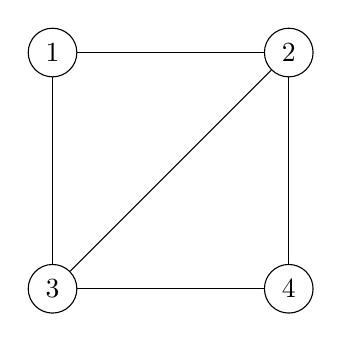
\begin{tikzpicture}[node distance={30mm}, main/.style = {draw, circle}] 
		\node[main] (1) {$1$}; 
		\node[main] (2) [right of=1] {$2$};
		\node[main] (3) [below of=1] {$3$};
		\node[main] (4) [below of=2] {$4$};
		\draw (1) -- (2);
		\draw (1) -- (3);
		\draw (2) -- (3);
		\draw (2) -- (4);
		\draw (3) -- (4);
	\end{tikzpicture}
	\caption{Primjer grafa s 4 vrha}
\end{figure}

Laplacian \textit{L} grafa sa slike 4.1 je:

\[
\centering
L = 
\begin{bmatrix}
	2 & -1 & -1 & 0 \\
	-1 & 3 & -1 & -1 \\
	-1 & -1 & 3 & -1 \\
	0 & -1 & -1 & 2
\end{bmatrix}
\]

Primjetimo da je suma svakog retka i stupca od \textit{L} jednak 0. Zbog toga je determinanta od \textit{L} uvijek jednaka 0.

Da bismo bili u mogućnosti iskazati matrični teorem o stablima, potrebno je uvesti još jedan komad notacije. Pretpostavimo li matricu \textit{A} s dimenzijama \textit{n} x \textit{n}, s \textit{A\textsuperscript{(ij)}} će se označavati matrica dimenzija (\textit{n} - 1) x (\textit{n} - 1) dobivena brisanjem \textit{i}-tog redka i \textit{j}-tog stupca matrice \textit{A}. Takve matrice se nazivaju \textit{minore}. Sljedeći teorem nam govori da nam minore \textit{Laplaciana} daju upravo rezultat koji tražimo.

\section{Matrix-Tree teorem}

\textbf{Matrix-Tree teorem:} \textit{Neka je G nepovezani graf ili multigraf i neka T(G) označava broj razapinjućih stabala u G. Za bilo koji i, T(G) = det L\textsuperscript{(ii)}, gdje je L laplacian od G. Preciznije, det L\textsuperscript{(ii)} je jednak za svaki i.}

\textbf{Dokaz:} Teorem se dokazuje matematičkom indukcijom. Pretpostavimo da teorem vrijedi za povezane grafove s manje vrhova ili bridova. Kao bazu indukcije, pretpostavimo da se graf \textit{G} sastoji od samo jednog vrha. U tom slučaju, $T(G) = 1$, i teorem daje ispravan rezultat: $L = (0)$ i $L^{(11)}$ je matrica dimenzija 0 x 0, čija je determinanta po definiciji jednaka 1.

Za korak indukcije pretpostavljamo graf \textit{G} koji ima barem dva vrha, te odabiremo jedan od tih vrhova, recimo vrh \textit{i}. Ako \textit{i} nije incidentan s nijednim bridom, onda \textit{G} nema razapinjuće stablo. U ovom slučaju će teorem vrijediti jer je \textit{L\textsuperscript{(ii)}} zapravo \textit{Laplacian} ostatka grafa te će njezina determinanta biti jednaka nuli, kao što je navedeno u odjeljku 4.1.

\begin{figure}[htb]
	\minipage{0.33\textwidth}
	\begin{center}
		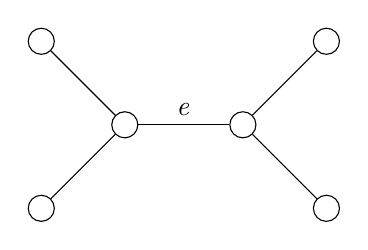
\begin{tikzpicture}[node distance={15mm}, main/.style = {draw, circle}] 
			\node[main] (1) {}; 
			\node[main] (2) [below right of=1] {};
			\node[main] (3) [right of=2] {};
			\node[main] (4) [above right of=3] {};
			\node[main] (5) [below left of=2] {};
			\node[main] (6) [below right of=3] {};
			\draw (1) -- (2);
			\draw (2) -- node[midway, above] {\textit{e}} (3);
			\draw (2) -- (5);
			\draw (3) -- (4);
			\draw (3) -- (6);
		\end{tikzpicture}
	\end{center}
	\caption*{\textit{G}}
	\endminipage\hfill
	\minipage{0.33\textwidth}
	\begin{center}
		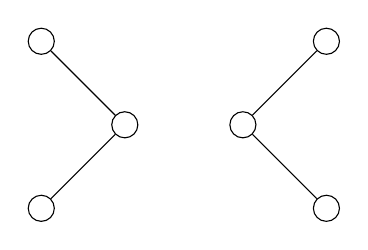
\begin{tikzpicture}[node distance={15mm}, main/.style = {draw, 	circle}] 
			\node[main] (1) {}; 
			\node[main] (2) [below right of=1] {};
			\node[main] (3) [right of=2] {};
			\node[main] (4) [above right of=3] {};
			\node[main] (5) [below left of=2] {};
			\node[main] (6) [below right of=3] {};
			\draw (1) -- (2);
			\draw (2) -- (5);
			\draw (3) -- (4);
			\draw (3) -- (6);
		\end{tikzpicture}
	\end{center}
	\caption*{\textit{G - e}}
	\endminipage\hfill
	\minipage{0.33\textwidth}
	\begin{center}
		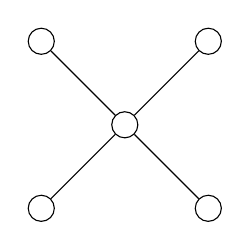
\begin{tikzpicture}[node distance={15mm}, main/.style = {draw, 	circle}] 
			\node[main] (1) {}; 
			\node[main] (2) [below right of=1] {};
			\node[main] (4) [above right of=2] {};
			\node[main] (5) [below left of=2] {};
			\node[main] (6) [below right of=2] {};
			\draw (1) -- (2);
			\draw (2) -- (5);
			\draw (2) -- (4);
			\draw (2) -- (6);
		\end{tikzpicture}
	\end{center}
	\caption*{$G \textbackslash e$}
	\endminipage\hfill
	\caption{$G - e$ je graf koji se dobije brisanjem brida \textit{e}, a $G \textbackslash e$ je graf koji se dobije kontrakcijom brida \textit{e} i spajanjem incidentnih vrhova u jedan vrh.}
\end{figure}

Sada pretpostavimo da je \textit{i} povezan s nekim drugim vrhom \textit{j}, te neka \textit{e} označava brid \textit{(i,j)}. Kao što je prikazano na slici 4.2, postoje dva načina na koje se može modificirati \textit{G}: brid \textit{e} možemo jednostavno izbrisati, ili možemo kontrakcijom vrhove \textit{i} i \textit{j} spojiti u jedan vrh. Takve grafove označujemo s $G - e$ i $G \textbackslash e$. Sada tvrdimo da je broj razapinjučih stabala \textit{T(G)} zadan sa sljedećim rekurzivnim izrazom:

\begin{equation}
	T(G) = T(G - e) + T(G \textbackslash e)
\end{equation}

Prije nastavka dokaza matričnog teorema o stablima potrebno je dokazati da je izraz (4.1) ispravan. Neka je \textit{e} neki fiksni brid od \textit{G}. Uočimo da se razapinjuća stabla od \textit{G} dijele na:
\begin{itemize}
	\item razapinjuća stabla od \textit{G} koja ne sadrže brid \textit{e}; neka je taj broj jednak x,
	\item razapinjuća stabla od \textit{G} koja sadrže brid \textit{e}; neka je taj broj jednak y.
\end{itemize}
Vrijedi: $T(G) = x + y$. Uočimo sada da je:
\begin{itemize}
	\item $x = T(G - e)$ jer je svako razapinjuće stablo od \textit{G} koje ne sadrži \textit{e}, ujedno i razapinjuće stablo od $G - e$
	\item $y = T(G \textbackslash e)$ jer svako razapinjuće stablo od $G \textbackslash e$ možemo dobiti iz razapinjućeg stabla od \textit{G} koje sadrži brid \textit{e} postupkom konkatenacije brida \textit{e} u tom stablu.
\end{itemize}
Dakle, vrijedi $T(G) = T(G - e) + T(G \textbackslash e)$.

Prtpostavimo sada da matrični teorem vrijedi za $G - e$ i za $G \textbackslash e$. Možemo razmjestiti vrhove od \textit{G} tako da su \textit{i} i \textit{j} prva dva vrha. Sada Laplacian \textit{L} od \textit{G} možemo napisati kao:

\[
L_G =
\begin{bmatrix}
	\begin{array}{c|c|c}
		d_i & -1 & r_i^T \\
		\hline
		-1 & d_j & r_j^T \\
		\hline
		r_i & r_j & L'
	\end{array}
\end{bmatrix}
\]

Ovdje \textit{r\textsubscript{i}} i \textit{r\textsubscript{j}} predstavljaju \textit{(n - 2)}-dimenzionalne vektore koji opisuju konekcije vrhova \textit{i} i \textit{j} s ostalih \textit{n - 2} vrha od \textit{G} ($r_i^T$ i $r_j^T$ su transponirani vektori), a \textit{L'} je \textit{(n - 2)}-dimenzionalna minora koja predstavlja \textit{laplacian} ostatka grafa. \textit{Laplaciane} grafova $G - e$ i $G \textbackslash e$ pišemo na sljedeći način:

\[
L_{G - e} = 
\begin{bmatrix}
	\begin{array}{c|c|c}
		d_i - 1 & 0 & r_i^T \\
		\hline
		0 & d_j - 1 & r_j^T \\
		\hline
		r_i & r_j & L'
	\end{array}
\end{bmatrix},
L_{G \textbackslash e} = 
\begin{bmatrix}
	\begin{array}{c|c}
		d_i + d_j - 2 & r_i^T + r_j^T \\
		\hline
		r_i + r_j & L'
	\end{array}
\end{bmatrix}
\]

Da bi se indukcija završila, potrebno je pokazati:

\begin{equation}
	detL_G^{(ii)} = detL_{G - e}^{(ii)} + detL_{G \textbackslash e}^{(jj)}
\end{equation}

ili, u matričnom zapisu:

\[
det
\begin{pmatrix}
	\begin{array}{c|c}
		d_j & r_j^T \\
		\hline
		r_j & L'
	\end{array}
\end{pmatrix}
= det
\begin{pmatrix}
	\begin{array}{c|c}
		d_j - 1 & r_j^T \\
		\hline
		r_j & L'
	\end{array}
\end{pmatrix}
+ detL'.
\]

Ovaj rezultat slijedi iz činjenice da determinanta matrice može biti napisana kao linearna kombinacija njenih \textit{kofaktora}, tj. determinanti njenih minora. Za bilo koju matricu \textit{A} vrijedi

\begin{equation}
	detA = \sum_{j = 1}^{n} (-1)^j A_{1,j} detA^{(1,j)}.
\end{equation}

Dakle, ako se dvije matrice razlikuju samo u njihovim (1,1) ćelijama, a $A_{ij} = B_{ij}$ za svaki drugi \textit{i} i \textit{j}, njihove determinante se razlikuju za determinantu njigovih (1,1) minora, odnosno $detA = detB + detA^{(1,1)}.$ Primjenimo li ovo za $L_G^{(ii)}$ i $L_{G - e}^{(ii)}$, dobit ćemo izraz (4.2), čime se dovršava dokaz ovog teorema.

\chapter{Računanje broja razapinjućih stabala pomoću matričnog teorema o stablima}

Da bismo se uvjerili da je rezultat prethodnog teorema zaista ispravan, u ovom poglavlju razraditi ćemo primjere.

\begin{figure}[htb]
	\centering
	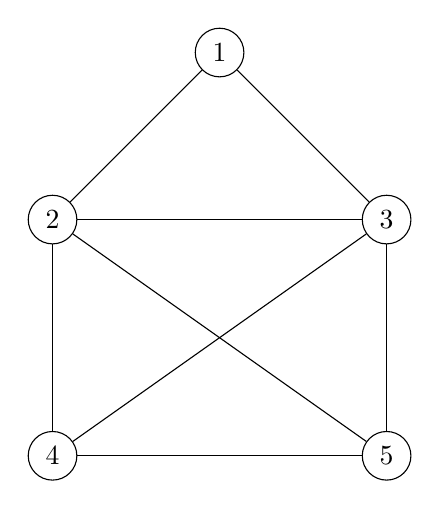
\begin{tikzpicture}[node distance={30mm}, main/.style = {draw, circle}] 
		\node[main] (1) {$1$}; 
		\node[main] (2) [below left of=1] {$2$};
		\node[main] (3) [below right of=1] {$3$};
		\node[main] (4) [below of=2] {$4$};
		\node[main] (5) [below of=3] {$5$};
		\draw (1) -- (2);
		\draw (1) -- (3);
		\draw (2) -- (3);
		\draw (2) -- (4);
		\draw (2) -- (5);
		\draw (3) -- (4);
		\draw (3) -- (5);
		\draw (4) -- (5);
	\end{tikzpicture}
	\caption{Primjer grafa s 5 vrhova}
\end{figure}

Na slici 5.1 prikazan je graf s 5 vrhova. Matrica susjedstva \textit{A} navedenog grafa, te njezin laplacian \textit{L} su sljedeći:

\[
\centering
A = 
\begin{bmatrix}
	0 & 1 & 1 & 0 & 0 \\
	1 & 0 & 1 & 1 & 1 \\
	1 & 1 & 0 & 1 & 1 \\
	0 & 1 & 1 & 0 & 1 \\
	0 & 1 & 1 & 1 & 0
\end{bmatrix}
,
L = 
\begin{bmatrix}
	2 & -1 & -1 & 0 & 0 \\
	-1 & 4 & -1 & -1 & -1 \\
	-1 & -1 & 4 & -1 & -1 \\
	0 & -1 & -1 & 3 & -1 \\
	0 & -1 & -1 & -1 & 3
\end{bmatrix}
\]

Kao sljedeći korak, stvorimo, na primjer, matricu \textit{L\textsuperscript{(22)}} dobivenu brisanjem drugog retka i drugog stupca matrice \textit{L}.

\[
\centering
L^{(22)} = 
\begin{bmatrix}
	2 & -1 & 0 & 0 \\
	-1 & 4 & -1 & -1 \\
	0 & -1 & 3 & -1 \\
	0 & -1 & -1 & 3
\end{bmatrix}
\]

Determinanta prethodne matrice, a ujedno i broj razapinjućih stabala grafa sa slike 5.1 je: $T(G) = det L^{(22)} = 40$. Jednak bi se rezultat dobio da smo matricu \textit{L\textsuperscript{(ii)}} stvorili tako da smo maknuli bilo koji drugi redak i stupac matrice \textit{L}.

\chapter{Graphelite - računanje broja razapinjućih stabala}

\chapter{Zaključak}
Zaključak.

\bibliography{literatura}
\bibliographystyle{fer}

\begin{sazetak}
Sažetak na hrvatskom jeziku.

\kljucnerijeci{Ključne riječi, odvojene zarezima.}
\end{sazetak}

% TODO: Navedite naslov na engleskom jeziku.
\engtitle{Title}
\begin{abstract}
Abstract.

\keywords{Keywords.}
\end{abstract}

\end{document}
